\documentclass[journal]{IEEEtran}
\usepackage[a5paper, margin=10mm]{geometry}
%\usepackage{lmodern} % Ensure lmodern is loaded for pdflatex
\usepackage{tfrupee} % Include tfrupee package

%iffalse
\let\negmedspace\undefined
\let\negthickspace\undefined
\usepackage{gvv-book}
\usepackage{gvv}
\usepackage{cite}
\usepackage{amsmath,amssymb,amsfonts,amsthm}
\usepackage{algorithmic}
\usepackage{graphicx}
\usepackage{textcomp}
\usepackage{xcolor}
\usepackage{txfonts}
\usepackage{listings}
\usepackage{enumitem}
\usepackage{mathtools}
\usepackage{gensymb}
\usepackage{comment}
\usepackage[breaklinks=true]{hyperref}
\usepackage{tkz-euclide} 
\usepackage{listings}                                        
%\def\inputGnumericTable{}                                 
\usepackage[latin1]{inputenc}                                
\usepackage{color}                                            
\usepackage{array}                                            
\usepackage{longtable}                                       
\usepackage{calc}                                             
\usepackage{multirow}                                         
\usepackage{hhline}                                           
\usepackage{ifthen}                                           
\usepackage{lscape}
\usepackage{tabularx}
\usepackage{array}
\usepackage{float}
\usepackage{multicol}

\newcommand{\BEQA}{\begin{eqnarray}}
\newcommand{\EEQA}{\end{eqnarray}}
%\newcommand{\define}{\stackrel{\triangle}{=}}

\setlength{\headheight}{1cm} % Set the height of the header box
\setlength{\headsep}{0mm}     % Set the distance between the header box and the top of the text


%\usepackage[a5paper, top=10mm, bottom=10mm, left=10mm, right=10mm]{geometry}


\setlength{\intextsep}{10pt} % Space between text and floats

% Marks the beginning of the document
\begin{document}
\onecolumn
\bibliographystyle{IEEEtran}
\vspace{3cm}

%\renewcommand{\theequation}{\theenumi}
\numberwithin{equation}{enumi}
\numberwithin{figure}{enumi}
\renewcommand{\thefigure}{\theenumi}
\renewcommand{\thetable}{\theenumi}

\title{GATE - EE - 2012 - 27 - 39}
\author{ai24btech11030 - Shiven Bajpai}
\maketitle

\iffalse
\begin{multicols}{4}
\begin{enumerate}
    \item 
    \item 
    \item 
    \item 
\end{enumerate}
\end{multicols}
\fi

\begin{enumerate}
   
    % Question 27
    \item The maximum value of \( f(x) = x^3 - 9x^2 + 24x + 5 \) in the interval \([1, 6]\) is

    \begin{multicols}{4}
        \begin{enumerate}
            \item $21$
            \item $25$
            \item $41$
            \item $46$
        \end{enumerate}
    \end{multicols}

    % Question 28
    \noindent
    \item{If \( V_A - V_B = 6 \, \text{V} \), then \( V_C - V_D \) is

    \begin{figure}[!ht]
        \centering
        \resizebox{0.6\textwidth}{!}{
        \begin{circuitikz}
        \tikzstyle{every node}=[font=\normalsize]
        \draw (7.5,14.25) to[R] (9.75,14.25);
        \draw (9.75,14.25) to[R] (11.75,14.25);
        \draw (11.75,14.25) to[R] (14,14.25);
        \draw [ line width=0.2pt](7.5,14.25) to[R] (7.5,12);
        \draw (9.75,14.25) to[R] (9.75,12);
        \draw (11.75,14.25) to[R] (11.75,12);
        \draw (11.75,12) to[R] (14,12);
        \draw (7.5,12) to[R] (9.75,14.25);
        \draw (11.75,12) to[R] (14,14.25);
        \draw (14,12) to[battery1] (14,14.25);
        \draw (7.5,12) to[battery1] (9.75,12);
        \draw (9.75,12) to[american current source] (11.75,12);
        \ctikzset{bipoles/resistor/height=0.15}
        \ctikzset{bipoles/resistor/width=0.4}
        \draw (10.25,12.75) to[R] (11.25,12.75);
        \draw (10.25,12.75) to[short] (10.25,12);
        \draw (11.25,12.75) to[short] (11.25,12);
        \node [font=\normalsize] at (7,13.25) {R};
        \node [font=\normalsize] at (8.5,14.75) {R};
        \node [font=\normalsize] at (8.25,13.5) {R};
        \node [font=\normalsize] at (9.25,12.75) {R};
        \node [font=\normalsize] at (12.75,14.75) {R};
        \node [font=\normalsize] at (12.75,11.5) {R};
        \node [font=\normalsize] at (13.25,12.75) {R};
        \node [font=\normalsize] at (10.75,13.25) {1$\Omega$};
        \node [font=\normalsize] at (10.5,14.75) {2$\Omega$};
        \node [font=\normalsize] at (12,13.25) {R};
        \node [font=\normalsize] at (14.75,13) {10V};
        \node [font=\normalsize] at (8.5,11.25) {5V};
        \node [font=\normalsize] at (10.75,11.25) {2A};
        \node [font=\normalsize] at (9.75,14.5) {$V_a$};
        \node [font=\normalsize] at (11.75,14.5) {$V_b$};
        \node [font=\normalsize] at (9.75,11.75) {$V_c$};
        \node [font=\normalsize] at (11.75,11.75) {$V_d$};
        \end{circuitikz}
        }
        
    \label{fig:my_label}
    \end{figure}

    \begin{multicols}{4}
        \begin{enumerate}
            \item \(-5 \, \text{V}\)
            \item \(2 \, \text{V}\)
            \item \(3 \, \text{V}\)
            \item \(6 \, \text{V}\)
        \end{enumerate}
    \end{multicols}}

    \item The voltage gain $A_v$ of the circuit shown below is

    \begin{center}
        
        \resizebox{0.4\textwidth}{!}{
        \begin{circuitikz}

        % Voltage source
        \draw (0,2) to[sinusoidal voltage source, l=$v_i$] (0,0.5) node[ground]{};
    
        % Coupling capacitor
        \draw (0,2) to[C, l=C] (2,2);
        
        % Transistor
        \draw (4,2) node[npn, anchor=B] (npn) {};
        \node at (5.5,1.5) {$\beta=100$};
        % \draw (4,1.5) to (5.5,1.5) node[ground]{};
        
        % Emitter resistor
        \draw (npn.E) -- ++(0,-0.75) node[ground]{};
        
        % Base resistor
        \draw (2,2) to[R, l=$10 \text{k}\Omega$] (4,2);
        \draw (npn.B) to[R, l=$100 \text{k}\Omega$] ++(0,+1.5) -- ++(0.85,0);
        
        % Collector resistor and supply voltage
        \draw (npn.C) -- ++(0,1) to[R, l=$12 \text{k}\Omega$] ++(0,1.5) -- ++(-0.5,0) -- ++(+1,0);
        \node at ($(npn.C)+(0,2.75)$) {13.7 Volts};
        
        % Output capacitor
        \draw (npn.C) to[C, l=C] (6,2.77) node[right] {$v_o$};
        
        \end{circuitikz}}
    \end{center}

    

    \begin{multicols}{4}
        \begin{enumerate}
            \item $\lvert A_v \rvert \approx 200$
            \item $\lvert A_v \rvert \approx 100$
            \item $\lvert A_v \rvert \approx 20$
            \item $\lvert A_v \rvert \approx 10$
        \end{enumerate}
    \end{multicols}

    \item {The state transition diagram for the logic circuit shown is

    \begin{center}
        \resizebox{0.4\textwidth}{!}{
        \begin{tikzpicture}
    
            % D Flip-Flop
            \draw (0,0) rectangle (2,2.5);
            \node at (0.25,1.9) {D};
            \node at (0.5,0.6) {CLK};
            \node at (1.5,0.6) {$\overline{Q}$};
            \node at (1.5,1.9) {Q};
        
            % MUX
            \draw (3,0) rectangle (5,2.5);
            \node at (3.5,1.9) {X1};
            \node at (3.5,0.6) {X0};
            \node at (4.75,1.25) {Y};
            \node at (4,0.25) {Select};
            \node at (4,2.75) {2-1 MUX};
        
            % Connections
            \draw[->] (-0.5,0.6) -- (0.1,0.6); % CLK arrow to D flip-flop
            \draw (2,1.9) -- (3,1.9); % Q to X1 of MUX
            \draw (2,0.6) -- (3,0.6); % /Q to X0 of MUX
            \draw (4,0) -- ++(0,-0.5) node[below] {A}; % Select line
            \draw (5,1.25) -- ++(0.5,0) -- ++(0,2) -- ++(-6.075,0) -- ++(0,-1.35) -- ++(0.575,0); % Feedback loop from Y output back to D input
        
        \end{tikzpicture}}
    \end{center}

    \begin{multicols}{2}
        \begin{enumerate}
            \item
                \resizebox{0.3\textwidth}{!}{
                \begin{tikzpicture}[->, >=stealth, node distance=2.5cm]
    
                % Nodes
                \node (q0) [circle, draw, minimum size=1.2cm] {Q=0};
                \node[right=of q0] (q1) [circle, draw, minimum size=1.2cm] {Q=1};
            
                % Self-loops
                \draw (q0) edge[loop above] node[above] {A=1} (q0);
                \draw (q1) edge[loop above] node[above] {A=0} (q1);
            
                % Transitions
                \draw (q0) edge[bend left] node[above] {A=1} (q1);
                \draw (q1) edge[bend left] node[below] {A=0} (q0);
            
            \end{tikzpicture}}
    
            \item
                \resizebox{0.3\textwidth}{!}{
                \begin{tikzpicture}[->, >=stealth, node distance=2.5cm]
    
                % Nodes
                \node (q0) [circle, draw, minimum size=1.2cm] {Q=0};
                \node[right=of q0] (q1) [circle, draw, minimum size=1.2cm] {Q=1};
            
                % Self-loops
                \draw (q0) edge[loop above] node[above] {A=0} (q0);
                \draw (q1) edge[loop above] node[above] {A=0} (q1);
            
                % Transitions
                \draw (q0) edge[bend left] node[above] {A=1} (q1);
                \draw (q1) edge[bend left] node[below] {A=1} (q0);
            
            \end{tikzpicture}}
    
            \item
                \resizebox{0.3\textwidth}{!}{
                \begin{tikzpicture}[->, >=stealth, node distance=2.5cm]
    
                % Nodes
                \node (q0) [circle, draw, minimum size=1.2cm] {Q=0};
                \node[right=of q0] (q1) [circle, draw, minimum size=1.2cm] {Q=1};
            
                % Self-loops
                \draw (q0) edge[loop above] node[above] {A=0} (q0);
                \draw (q1) edge[loop above] node[above] {A=1} (q1);
            
                % Transitions
                \draw (q0) edge[bend left] node[above] {A=0} (q1);
                \draw (q1) edge[bend left] node[below] {A=1} (q0);
            
            \end{tikzpicture}}
    
            \item
                \resizebox{0.3\textwidth}{!}{
                \begin{tikzpicture}[->, >=stealth, node distance=2.5cm]
    
                % Nodes
                \node (q0) [circle, draw, minimum size=1.2cm] {Q=0};
                \node[right=of q0] (q1) [circle, draw, minimum size=1.2cm] {Q=1};
            
                % Self-loops
                \draw (q0) edge[loop above] node[above] {A=1} (q0);
                \draw (q1) edge[loop above] node[above] {A=1} (q1);
            
                % Transitions
                \draw (q0) edge[bend left] node[above] {A=0} (q1);
                \draw (q1) edge[bend left] node[below] {A=0} (q0);
            
            \end{tikzpicture}}
    
        \end{enumerate}
    \end{multicols}
    }

    \item Let $y[n]$ denote the convolution of $h[n]$ and $g[n]$, where $h[n] = (1/2)^n u[n]$ and $g[n]$ is a causal sequence. If $y[0]=1$ and $y[1] = 1/2$, then $g[1]$ equals

    \begin{multicols}{4}
        \begin{enumerate}
            \item $0$
            \item $\frac{1}{2}$
            \item $1$
            \item $\frac{3}{2}$
        \end{enumerate}
    \end{multicols}

    \item The circuit shown is a

    \begin{center}
        \begin{circuitikz}
            \ctikzset{bipoles/length=1cm}
            \ctikzset{bipoles/capacitor/height=0.4}
            \ctikzset{bipoles/capacitor/width=0.1}
            \draw
            (0, 0) node[op amp] (opamp) {}
            (opamp.-) to[R,l_=$R_1$] (-2, 0.35) to[C,l=C] (-3, 0.35)
            (opamp.-) to[short,*-] ++(0,0.5) coordinate (leftC)
            to[R=$R_2$] (leftC -| opamp.out)
            to[short,-*] (opamp.out) to [short,-o] (1.5,0)
            (opamp.+) -- (-1,-0.35) to (-1,-0.5) node[ground]{};
            \node at (-3,-0) [ground]{} -- ++(0,1);
            \node at (1.5,-0.5) [ground]{};
            \node [font=\small] at (-3.5,0) {Input};
            \node [font=\small] at (2,-0.25) {Output};
        \end{circuitikz}
    \end{center}

    \begin{enumerate}
        \item low pass filter with $f_{3\text{dB}} = \frac{1}{(R_1 + R_2)C}$ rad/s
        \item high pass filter with $f_{3\text{dB}} = \frac{1}{R_1 C}$ rad/s
        \item low pass filter with $f_{3\text{dB}} = \frac{1}{R_1 C}$ rad/s
        \item high pass filter with $f_{3\text{dB}} = \frac{1}{(R_1 + R_2)C}$ rad/s
    \end{enumerate}

    \item For the system shown below, $S_{D1}$ and $S_{D2}$ are complex power demands at bus 1 and bus 2 respectively. If $\lvert V_2 \rvert = 1 \, \text{pu}$, the VAR rating of the capacitor $(Q_{G2})$ connected at bus 2 is

    \begin{center}
        \centering
        \resizebox{0.4\textwidth}{!}{%
        \begin{circuitikz}
        \tikzstyle{every node}=[font=\small]
        \ctikzset{bipoles/capacitor/height=0.4}
        \ctikzset{bipoles/capacitor/width=0.1}
        \draw (8,13) to[sinusoidal voltage source, sources/symbol/rotate=auto] (10,13);
        \draw [ line width=0.9pt](10,13.75) to[short] (10,12.25);
        \draw [ line width=0.2pt](10,13.5) to[short] (12.25,13.5);
        \draw [ line width=0.2pt](10,12.5) to[short] (10.5,12.5);
        \draw [ line width=1.1pt](12.25,13.75) to[short] (12.25,12.25);
        \draw [ line width=0.2pt](12.25,12.5) to[short] (11.75,12.5);
        \draw [line width=0.2pt, ->, >=Stealth] (10.5,12.5) -- (10.5,11.75);
        \draw [line width=0.2pt, ->, >=Stealth] (11.75,12.5) -- (11.75,11.75);
        \draw [line width=0.2pt, short] (12.25,13) -- (12.75,13);
        \draw [line width=0.2pt](12.75,13) to[C] (12.75,12.25);
        \node at (12.75,12.25) [ground]{};
        \node [font=\normalsize] at (8.4,13.5) {$S_{G1}$};
        \node [font=\small] at (10,14) {$v_1 = 1/0 pu$};
        \node [font=\small] at (10,14.35) {$Bus 1$};
        \node [font=\small] at (12.25,14) {$V_2$};
        \node [font=\small] at (12.25,14.35) {$Bus 2$};
        \node [font=\small] at (13.1,13) {$Q_{G2}$};
        \node [font=\small] at (10,11.5) {$S_{D1} = 1pu$};
        \node [font=\small] at (12.25,11.5) {$S_{D2} = 1 pu$};
        \node [font=\small] at (11,13.25) {$Z = j \: 0.5 pu$};
        \end{circuitikz}
        }%
    \end{center}

    \begin{multicols}{4}
        \begin{enumerate}
            \item $0.2$ pu
            \item $0.268$ pu
            \item $0.312$ pu
            \item $0.4$ pu
        \end{enumerate}
    \end{multicols}

    \item A cylindrical rotor generator delivers 0.5 pu power in the steady-state to an infinite bus through a transmission line of reactance 0.5 pu. The generator no-load voltage is 1.5 pu and the infinite bus voltage is 1 pu. The inertia constant of the generator is 5 MW-s/MVA and the generator reactance is 1 pu. The critical clearing angle, in degrees, for a three-phase dead short circuit fault at the generator terminal is

    \begin{multicols}{4}
        \begin{enumerate}
            \item $53.5$
            \item $60.2$
            \item $70.8$
            \item $79.6$
        \end{enumerate}
    \end{multicols}

    \item In the circuit shown, an ideal switch $S$ is operated at 100 kHz with a duty ratio of 50\%. Given that $\Delta i_c$ is 1.6 A peak-to-peak and $I_0$ is 5 A dc, the peak current in $S$ is

    \begin{figure}[!ht]
        \centering
        \resizebox{0.5\textwidth}{!}{%
        \begin{circuitikz}
        \tikzstyle{every node}=[font=\small]
        \ctikzset{bipoles/capacitor/height=0.4}
        \ctikzset{bipoles/capacitor/width=0.1}
        \ctikzset{bipoles/resistor/height=0.15}
        \ctikzset{bipoles/resistor/width=0.4}
        \ctikzset{bipoles/diode/height=0.2}
        \ctikzset{bipoles/diode/width=0.2}
        \draw (10,13.5) to[battery1, l=24 V] (10,12.25);
        \draw [line width=0.2pt](10,13.5) to[normal open switch, l=S] (12,13.5);
        \draw [ line width=0.2pt](12,12.25) to[D, l=D] (12,13.5);
        \draw [ line width=0.2pt](10,12.25) to[short] (15,12.25);
        \draw [line width=0.2pt](12,13.5) to[L, l=L] (14,13.5);
        \draw [line width=0.2pt](14,13.5) to[C,l=C] (14,12.25);
        \draw [ line width=0.2pt](15,13.5) to[R, l=R] (15,12.25);
        \draw [ line width=0.2pt](14,13.5) to[short] (15,13.5);
        \node [font=\small] at (15,13.75) {$I_0$};
        \node [font=\small] at (13.75,13.25) {$\Delta i_0$};
        \node [font=\small] at (15.5,12.875) {$v_0$};
        \draw [line width=0.2pt, ->, >=Stealth] (15.5,12.625) -- (15.5,12.25);
        \draw [line width=0.2pt, ->, >=Stealth] (15.5,13.125) -- (15.5,13.5);
        \end{circuitikz}
        }%
        
    \label{fig:my_label}
    \end{figure}

    \begin{multicols}{4}
        \begin{enumerate}
            \item $6.6$ A
            \item $5.0$ A
            \item $5.8$ A
            \item $4.2$ A
        \end{enumerate}
    \end{multicols}

    \item A 220 V, 15 kW, 1000 rpm shunt motor with armature resistance of $0.25\,\Omega$, has a rated line current of 68 A and a rated field current of 2.2 A. The change in field flux required to obtain a speed of 1600 rpm while drawing a line current of 52.8 A and a field current of 1.8 A is

    \begin{multicols}{2}
        \begin{enumerate}
            \item $18.18 \%$ increase
            \item $18.18 \%$ decrease
            \item $36.36 \%$ increase
            \item $36.36 \%$ decrease
        \end{enumerate}
    \end{multicols}

    \item A fair coin is tossed till a head appears for the first time. The probability that the number of required tosses is odd, is

    \begin{multicols}{4}
        \begin{enumerate}
            \item $\frac{1}{3}$
            \item $\frac{1}{2}$
            \item $\frac{2}{3}$
            \item $\frac{3}{4}$
        \end{enumerate}
    \end{multicols}

    \item The direction of vector $\vec{A}$ is radially outward from the origin, with $\lvert \vec{A} \rvert = kr^n$ where $r^2 = x^2 + y^2 + z^2$ and $k$ is a constant. The value of $n$ for which $\nabla \cdot \vec{A} = 0$ is

    \begin{multicols}{4}
        \begin{enumerate}
            \item $-2$
            \item $2$
            \item $1$
            \item $0$
        \end{enumerate}
    \end{multicols}

    \item Consider the differential equation
    $$ \frac{d^2 y(t)}{dt^2} + 2 \frac{dy(t)}{dt} + y(t) = \delta(t) \quad \text{with} \left. \quad y(t) \right|_{t=0^{-}} = -2 \quad \text{and} \quad \left. \frac{dy}{dt} \right|_{t=0^{-}} = 0. $$
    The numerical value of $\left. \frac{dy}{dt} \right|_{t=0^{+}}$ is

    \begin{multicols}{4}
        \begin{enumerate}
            \item $-2$
            \item $-1$
            \item $0$
            \item $1$
        \end{enumerate}
    \end{multicols}

\end{enumerate}
\end{document}

